\section{Die Streifenmethode} \label{streifen}
\begin{figure}[h]
	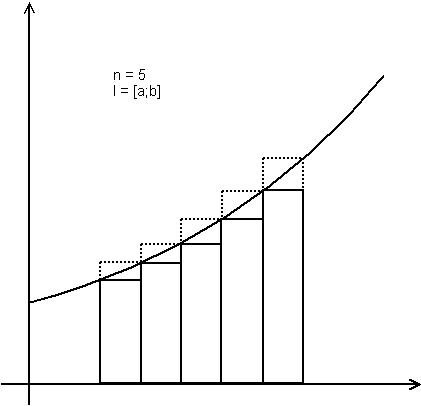
\includegraphics[width=0.75\textwidth]{abbildungen/int1.jpg}
	\caption{Streifenmethode}
	\label{fig:int1}
\end{figure}
\begin{itemize}
	\item Einbeschriebene Rechteckfl�chen $\rightarrow$ Untersumme $U_5$
	\item Umbeschriebene Rechteckfl�chen $\rightarrow$ Obersumme $O_5$
	\item Verfeinerung der Intervalleinteilung auf n gleiche Intervallabschnitte $U_n$, $O_n$
	\item $n \rightarrow \infty$
	\item ${\lim}_{n \rightarrow \infty} [U_n] = {\lim}_{n \rightarrow \infty} [O_n] = A^b _a$
\end{itemize} 
\begin{bsp}
$ f(x) = x$ \\
\begin{figure}[h]
	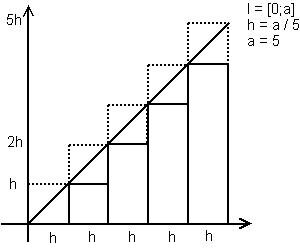
\includegraphics[width=1.00\textwidth]{abbildungen/int2.jpg}
	\caption{$f(x) = x$}
	\label{fig:int2}
\end{figure}
\end{bsp}

\textbf{Einschub \ref{streifen}.1:} Das Summenzeichen
\begin{align*}
1+2+3+4 &= \sum \limits_{\nu = 1}^4 \nu = 10 \\
1+2+3+4+...+n &= \sum \limits_{\nu = 1}^n \nu \\
\end{align*}

\begin{align*}
&U_5 = 1hh +2hh+3hh+4hh = h^2 \cdot (1+2+3+4) = \frac{a^2}{5^2} \cdot \sum \limits_{\nu = 1}^4 \nu \\
&O_5 = 1hh +2hh+3hh+4hh+5hh = h^2 \cdot (1+2+3+4+5) = \frac{a^2}{5^2} \cdot \sum \limits_{\nu = 1}^5 \nu \\
&U_n = \frac{a^2}{n^2} \cdot \sum \limits_{\nu = 1}^{n-1} \nu \\
&O_n = \frac{a^2}{n^2} \cdot \sum \limits_{\nu = 1}^{n} \nu \\
\end{align*}


\textbf{Einschub \ref{streifen}.2:} \\
$\sum \limits_{\nu = 1}^{n} \nu = \frac{n(n+1)}{2}$\\


\begin{align*}
U_n &= \frac{a^2}{n^2} \cdot \frac{(n-1)n}{2}\\
&= \frac{a^2}{2} \cdot \frac{n^2-n}{n^2}\\
O_n &= \frac{a^2}{n^2} \cdot \frac{n(n+1)}{2}\\
&= \frac{a^2}{2} \cdot \frac{n^2+n}{n^2}\\
\lim_{n \to \infty} U_n &= \lim_{n \to \infty} \left[\frac{a^2}{2} \cdot \frac{n^2-n}{n^2}\right]\\
&= \lim_{n \to \infty}\left[\frac{a^2}{2} \cdot (1-\frac{1}{n})\right] = \frac{a^2}{2}\\
\lim_{n \to \infty} O_n &= \lim_{n \to \infty} \left[\frac{a^2}{2} \cdot \frac{n^2+n}{n^2}\right]\\
&= \lim_{n \to \infty}\left[\frac{a^2}{2} \cdot (1+\frac{1}{n})\right] = \frac{a^2}{2}
\end{align*}
\\
F�r $ f(x) = x$ gilt also $A^a _0 = \frac{a^2}{2}$ also $A_a ^b = A_0^b - A_0^a = \frac{b^2}{2} - \frac{a^2}{2}$ \\
entsprechend gilt f�r $f(x) = x^2$: $A_0^a = \frac{a^3}{3}$ und so weiter... 

\section{Stammfunktionen}
$F(x) = \frac{x^2}{2} \rightarrow F'(x) = f(x)$\\
$F(x)$ ist die Stammfunktion von $f(x)$ \\
\begin{definition}[Stammfunktion] Eine differenzierbare Funktion $F$ hei�t \textbf{Stammfunktion} zu einer Funktion $f$, genau dann wenn gilt: $F'(x)  =f(x)$
\end{definition}
\begin{tabular}{l|l}
\hline
\textbf{Funktion} & \textbf{Stammfunktion} \\
\hline
$f(x) = x^2$ & $F(x) = \frac{1}{3} x^3$ oder $G_{17} (x)= \frac{1}{3} x^3 + 17$ oder $G_c (x) = F(x) + c$ \\ \hline
\end{tabular}
\\
\\
$A_a ^b= \frac{1}{3} x^3 +5 ]^b _a = \frac{1}{3} b^3 + 5 - (\frac{1}{3} a^3 + 5)$ \\
\\
Stammfunktion $F$ $\rightarrow$ unendliche viele \\
Grundfunktion $f$ \\
Ableitungsfunktion $f'$ $\rightarrow$ eindeutig
\subsection {Eigenschaften von Stammfunktionen}
(Ziel: Bildung von Stammfunktionen folgender Funktionen) \\
(Voraussetzung: $U$ Stammfunktion von $u$, $V$ Stammfunktion von $v$) 
\\
\begin{tabular}{l|l}
\textbf{Funktion} & \textbf{Stammfunktion} \\ \hline
$f(x) = x^n \land n \in \mathbb{R}^{\neq-1}$ & $F(x) = \frac{1}{n+1} \cdot x^{n+1}$ \\ \hline
$f(x) = c \cdot u(x)$ & $F(x) = c \cdot U(x)$ \\ \hline
$f(x) = u(x) + v(x)$ & $F(x) = U(x) + V(x)$ \\ \hline
$f(x) = x^{-1}$ & noch nicht mglich \\ \hline
$f(x) = u(x) \cdot v(x)$ & noch nicht m�glich \\ \hline
$f(x) = u(rx + b)$ (lineare Verkettung) & $F(x) = \frac{1}{r} U (rx+b)$ \\ \hline
\end{tabular}

\section{Bestimmte Integrale}
Beliebige Funktion $f$ (stetig, d.h. "`ohne L�cke und Sprung"') \\
Unterteilt in $n$ gleiche Teilintervalle $[a,b]$ der Breite $\Delta x$ \\
\begin{align*}
&U_n = \sum \limits_{\nu = 0}^{n-a} f(a+ \nu \Delta x) \Delta x \\
&O_n = \sum \limits_{\nu = 1}^{n} f(a+ \nu \Delta x) \Delta x  \\
&\lim_{n \to \infty} U_n = \int \limits_{a}^{b} f(x)dx \\
&\lim_{n \to \infty} O_n = \int \limits_{a}^{b} f(x)dx\\
\end{align*}

\subsection{Eigenschaften des bestimmten Integrals}
\begin{enumerate}
	\item $\int \limits_{a}^{a} f(x) dx = 0$
	\item Faktorregel: $k \cdot \int \limits_{a}^{b} f(x) dx = \int \limits_{a}^{b} k \cdot f(x) dx$
	\item Summenregel: $\int \limits_{a}^{b} f(x) + g(x) dx = \int \limits_{a}^{b} f(x) dx + \int \limits_{a}^{b} g(x) dx$
	\item Grenzen vertauschen: $\int \limits_{a}^{b} f(x) dx = -\int \limits_{b}^{a} f(x) dx$
	\item Intervalladditivit�t: $\int \limits_{a}^{b} f(x) dx = \int \limits_{a}^{c} f(x) dx + \int \limits_{c}^{b} f(x) dx$ wenn $a<c<b$
	\item Monotonie des Integrals: \\ $f(x) \leq g(x)$ auf $I = [a,b] \Rightarrow \int \limits_{a}^{b} f(x) dx \leq \int \limits_{a}^{b} g(x) dx$
	\item $\int \limits_{a}^{b} f(x) dx = \int \limits_{a}^{b} f(t) dt$
	\item falls $f(-x) = -f(x) \land x \in I=[a,b]$ dann $\int \limits_{-a}^{a} f(x) dx = 0$
\end{enumerate}

\section {Fl�che zwischen Graph und x-Achse}
Wenn der Graph auf $I=[a,b]$ \emph{keine} Nullstelle besitzt, dann errechnet man die Fl�che wie folgt: \\
$A =  \left| \int \limits_{a}^{b} f(x) dx \right|$ \\
Besitzt der Graph auf $I=[a,b]$ Nullstellen, so muss der Intervall in Teilintervalle unterteilt werden. Sei zum Beispiel $c$ die (einzige) Nullstelle von $f(x)$. Dann ist die Fl�che $A= \left| \int \limits_{a}^{c} f(x) dx \right| + \left| \int \limits_{c}^{b} f(x) dx \right|$

\section{Fl�che zwischen zwei Graphen}
\subsection{... die sich auf [a,b] nicht schneiden}
$A= \left| \int \limits_{a}^{b} f(x) - g(x) dx \right|$
\subsection{... die sich auf [a,b] schneiden}
\begin{enumerate}
	\item Schnittpunkte berechnen
	\item Teilfl�chen berechnen
	\item Teilfl�chen aufaddieren
\end{enumerate}

\section{Menge aller Integralfunktionen}
$I_a (x) = \int \limits_{a}^{x} f(x) dx = F(x)]^x_a=F(x) - F(a)$

\section{Hauptsatz der Integral und Differentialrechnung}
\begin{satz}[Hauptsatz der Integral- und Differentialrechnung]
Sei $f$ eine auf $I=[a,b]$ stetige Funktion. Dann gilt f�r die Funktion $I_a$ mit $I_a = \int \limits_{a}^{x} f(t) dt$:
\begin{align*}
I'_a (x) &= f(x) \\
\int \limits_{a}^{b} f(x) dx &= F(b) - F(a) \in \mathbb{R}
\end{align*}
\end{satz}

\section{Einschub: Vollst�ndige Induktion (LK)} \label{vollind}
\emph{Axiom von Peano:}\\
$M$ Menge. \\
\begin{align*}
1 \in M \land (n \in M \Rightarrow n+1 \in M) \Rightarrow M = \mathbb{N}
\end{align*}
\\
\begin{bsp}
Summe aller ungeraden Zahlen: $ 1+3+5+...+(2n-1) = n^2$
\begin{beweis}

\begin{enumerate}
	\item Verankerung: \\ 
	$A_{(1)}$ ist wahr, denn $1 = 1^2$
	\item Schluss von $n$ auf $n+1$: \\
	$A_{(n+1)}$ ist wahr unter Verwendung der Wahrheit von $A_(n)$ \\
	$A_{(n+1)}$: \\
	$1+3+5+...+(2(n+1)-1) = (n+1)^2$ \\
	$\Leftrightarrow 1+3+5+...+(2n-1) + (2(n+1)-1) = (n+1)^2$ \\
	$\Leftrightarrow n^2 + (2(n+1)-1)=(n+1)^2$\\
	$\Leftrightarrow n^2 + 2n + 1 = (n+1)^2$ \\
	$\Leftrightarrow (n+1)^2 = (n+1)^2$
	\item Nach Peano Axiom gilt damit: $A_{(n)} \forall n \in \mathbb{N}$
\end{enumerate}
\end{beweis}
\end{bsp}

\section{Rotationsk�rper (LK)}
... sind K�rper, die durch die Rotation einer Fl�che um eine Achse entstehen. \\
Ziel: Berechnung des Volumens mit Hilfe der Integralrechnung. \\
\\
Sei $f$ auf $I=[a,b]$ stetig. \\
Gesamtvolumen $\rightarrow$ unendlich viele Zylinder.
\begin{align*}
V&= \lim_{n \to \infty}  \sum \limits_{}^{n-1} \pi f^2(x) dx\\
&= \pi \int \limits_{a}^{b} f^2(x) dx
\end{align*}
= Volumen eines Rotationsk�rper, der durch $f$ erzeugt wird. \\
Wird z.B. benutzt, um das Volumen einer Kugel herzuleiten! \\
F�r einen Rotationsk�rper, der von zwei Funktionen vorgegeben wird, gilt:
\begin{align*}
V&= \pi \int \limits^{b}_{a} f^2(x)dx - \pi \int \limits^{b}_{a} g^2(x)dx \\
&= \pi \int \limits^{b}_{a} f^2(x) - g^2(x)dx
\end{align*}


\section{Weitere Integrationsregeln (LK)}


\subsection{Partielle Integration}
Dient zum Integrieren von Produkten von Funktionen. \\
Produktregel: $(u(x) \cdot v(x))' = v'(x) u(x) + u'(x) v(x)$ $u, v$ differenzierbar und stetig; $u', v'$ stetig \\
\begin{align*}
u(x) v'(x) &= (u(x) v(x))' - u'(x) v(x) \\
\Leftrightarrow \int \limits_{a}^{b} {u(x) v'(x)dx} &= \int \limits_{a}^{b} {(u(x) v(x))' dx} - \int \limits_{a}^{b} {u'(x)v(x)dx}
\end{align*}
Dies f�hrt zu folgender Regel zum Integrieren von Produkten von Funktionen:
\begin{align}
\int \limits_{a}^{b} {u(x) v'(x)dx} = u(x) \cdot v(x) ]_a ^b - \int \limits_{a}^{b} {u'(x)v(x)dx}
\end{align}


\subsection{Integration durch Substitution}
(Basiert auf der Kettenregel der Differentialrechnung) \\
Kettenregel: \\
$u \circ v(x) = u(v(x))$; u, v diffbar \\
$(u \circ v(x)') = (u(v(x)))' = u'(v(x) \cdot v'(x))$ \\

Sei $U$ Stammfunktion von $u$: $U'(x) = u(x)$
\begin{align*}
(U(x))' &= U'(v(x)) \cdot v'(x) = u(v(x) \cdot v'(x)\\
\Rightarrow \int \limits_{a}^{b} {u(v(x)) \cdot v'(x)}dx &= \int \limits_{a}^{b} {U'(v(x))}dx = U(v(x))]_a ^b = U(v(b)-U(v(a))
\end{align*}

Substitution: $ = U(z)]_{v(a)}^{v(b)}$ \\
Daraus ergibt sich folgende Regel:
\begin{align}
\int \limits_{a}^{b} {u(v(x)) \cdot v'(x)}dx = U(z)]_{v(a)}^{v(b)}
\end{align}